\hyphenation{
Barrow
Binet
Chebyshev
Cholesky
Cramer
Gauss
Faber
Hausdorff
Householder
Laplace
Lebesque
Newton
Rolle
Runghe
Sturm
tras-for-ma-zio-ne
Torricelli
}


\chapter{Sistema Floating Point.}

\section{Definizione di un sistema Floating Point.}
\begin{defi}(Sistema Floating Point)
Siano $\beta$, $t$, $m$ ed $M$ interi positivi tale che:
$\beta \geq 2, \quad t \geq 1, \quad m,n > 0.$ L'insieme dei numeri macchina
in base $\beta$ con $t$ cifre significative è l'insieme:
\[F(\beta, t, m, M) = \{0\} \cup \left\{x \in \rr \colon x = \textrm{sgn}(x)
\cdot \sum_{i = 1}^{t}d_i\beta^{-i}\cdot \beta^p\right\},\]
tale che:
\begin{itemize}
\item[-]$0 \leq d_i < \beta, \qquad i = 1, \ldots, t.$
\item[-]$d_1 \neq 0.$
\item[-]$-m \leq p \leq M$.
\end{itemize}
\end{defi}

\begin{osse}Se $x$ appartiene ad un formato floating point può essere
espresso mediante un finito numero di cifre.
\[x \in F(\beta, t, m, M), \ x \neq 0 \ \Rightarrow \ x = \pm (.
\underbrace{d_1\cdots d_t}_{\textrm{finite}}
)_{\beta}\cdot \beta^p.\]
\end{osse}

\begin{exe}
Prendiamo il seguente sistema floating point e vediamo alcuni esempi:\\

$F(2,3,1,1)$
\[\beta = 2, \quad t = 3, \quad m = 1, \quad M = 1,\]

$d_1 = 1$, poiché non può essere uguale a zero.
\begin{itemize}
\item[]$(.100)_2 = \frac{1}{2}$;
\item[]$(.101)_2 = \frac{1}{2} + \frac{1}{8} = \frac{5}{8}$;
\item[]$(.110)_2 = \frac{1}{2} + \frac{1}{4} = \frac{3}{4}$;
\item[]$(.111)_2 = \frac{1}{2} + \frac{1}{4} + \frac{1}{8} = \frac{7}{8}$.
\end{itemize}
Queste di cui sopra sono alcune delle mantisse del sistema, le possibili
caratteristiche sono $-1$, $0$ e $1$ poiché $-1 \leq p \leq 1$.
\[F(2,3,1,1) = \left\{0, \frac{1}{4}, \pm\frac{9}{16}, \pm\frac{3}{8}, 
\pm\frac{7}{16}, \pm\frac{1}{2}, \pm\frac{9}{8}, \pm\frac{3}{4}, 
\pm\frac{7}{8}, \pm 9, \pm\frac{9}{4}, \pm\frac{3}{2}, \pm\frac{7}{4}
\right\}.
\]
\end{exe}
I numeri sono equispaziati fra la successione potenze della base, ma non in 
tutto il range.

\section{Proprietà.}
Sia $F(\beta, t, m, M)$ un sistema floating point, allora valgono le seguenti
proprietà:

\begin{enumerate}
\item
La cardinalità di $F(\beta, t, m, M)$ è esprimibile come:
\[2 \cdot \left(m + M + 1\right) \cdot \left( \beta -1\right)
\cdot \beta^{t-1} +1.\]
$2$ è dato dal segno, ogni numero può essere negativo o positivo (tutti i
numeri nel formato hanno opposto). $(m + M + 1)$ è il numero dei valori che
può assumere il peso $p$. $(\beta -1)\cdot \beta^{t-1}$ è il numero dei
valori che può assumere la mantissa. $1$ è dato dalla rappresentazione di $0$.
\item
I numeri macchina sono equispaziati fra le successive potenze di $\beta$ ma
non in tutto il range.
\item
Il più piccolo numero rappresentabile è:
\[(.1\,0\, \cdots \,0)_{\beta}\cdot \beta^{-m} = \beta^{-m - 1}.\]
(\verb1realmin1)
\item
Il più grande numero rappresentabile è:
\[\underbrace{(.\beta-1\, \beta-1 \, \cdots \, \beta-1)_{\beta}}_{1-\beta^{-t}}
\cdot  \beta^{M} \backsimeq\footnote{$t$ molto grande.} \beta^{M}.\]
(\verb1realmax1)
\end{enumerate}

\section{Il sistema Floating Point usato da Matlab.}

\begin{defi}
Sia un sistema Floating Point tale che:
\begin{itemize}
\item[-]$\beta = 2$;
\item[-]posti $p \in \zz$, $\,d_0 = 1$, $\,d_i = \verb1bit1$, $\,(i \geq 1)\,$
e $d_i$ definitivamente diverso da $1$,
\[x \in \rr \setminus \{0\} \ \Rightarrow \ x = \pm \sum_{i=0}^{+\infty}
d_i 2^{-i}
\cdot 2^p.\]
\end{itemize}
si dice che utilizza una rappresentazione \emph{normalizzata}. Ovvero $x$ si
può così definire:
\[
\begin{array}{lcl}
x & = & \pm \left(1 +  \sum_{i=1}^{+\infty}d_i2^{-1} \right)\cdot 2^p \\
  & = & \pm \left(1.d_1\,d_2\,\ldots\, \right)\cdot 2^p \\
  & = & \pm (1 + f)\cdot 2^p \qquad \textrm{con } 0 \leq f < 1.
\end{array}
\]
\end{defi}
Un formato che utilizza una forma normalizzata si denota con $F^*$.
\begin{exe}
$F^*(2,t,m,M) = \{0\} \cup \left\{ x \in \rr \colon\ x = \pm
(1 +  \sum_{i=1}^{t}d_i2^{-1})\cdot 2p\right\}$, con $d_i = \verb1bit1$,
$\ 1 \leq i \leq t\ $ e $\ -m \leq p \leq M$.
\end{exe}

Alcuni possibili formati sono:
\begin{itemize}
\item[] Singola precisione: $F^*(2,23,128,127);$
\item[] Doppia precisione: $F^*(2,52,1024,1023).$
\end{itemize}

Matlab utilizza un sistema Floating Point conforme allo standard IEEE-754
a doppia precisione, ovvero del tipo $F^*(2,52,1024,1023)$, ogni numero occupa
$64$ bit ($8$ byte).

\section{Numeri macchina e rappresentazione dei reali.}
L'insieme $F^*(2,52,1024,1023)$, detto insieme dei numeri macchina, è finito,
questo implica che dato un numero reale $x \in \rr$, questo possa appartenere
o meno all'insieme dei numeri macchina.

Se tale $x$ appartiene all'insieme dei numeri macchina non ci sono problemi
(saremmo comunque molto fortunati), la norma è che $x$ non vi appertenga.
Che errore commettiamo rappresentando $x \in \rr$ tale che $x \notin F$?
\begin{flushleft}
Sia $x \in \rr^+$, $\, x \notin F(\beta,t,m,M)$, allora:
\[x = \beta^p \sum_{i = 1}^{\infty}d_i \beta^{-i}.\]
Problema: come si associa in modo adeguato ad $x$ un numero di macchina
$\tilde{x} \in F(\beta,t,m,M)$?
\end{flushleft}
Distinguiamo due casi:
\begin{itemize}
\item[a)] $p \notin [-m,M]$
  \begin{enumerate}
  \item $p < -m \ \longrightarrow \ \textrm{UNDERFLOW}\qquad \tilde{x} = 0$;
  \item $p > M \ \longrightarrow \ \textrm{OVERFLOW} \qquad 
    \nexists\, \tilde{x}$, in questo caso o si arresta il calcolo oppure si
    imposta $\tilde{x} = \verb1Inf1$.
  \end{enumerate}
\item[b)]$p \in [-m,M]$, ma $\exists i > t \colon d_i \neq 0$
\begin{enumerate}
  \item Troncamento di $x$ alla $t$-esima cifra:
\[\tilde{x} = \textrm{trn}(x) = \beta^p \sum_{i=1}^td_i\beta^{-i}.\]
  \item Arrotondamento di $x$ alla $t$-esima cifra:
\[\tilde{x} = \textrm{arr}(x) = \beta^p \textrm{trn}\left(
\sum_{i=1}^{t+1}d_i\beta^{-i} + \frac{\beta}{2}\beta^{-t-1}\right).\]
  \end{enumerate}
\end{itemize}


Possiamo notare che se $d_{i+1} < \frac{\beta}{2}$ allora $\textrm{arr}(x)
= \textrm{trn}(x)$, se invece $d_{i+1} > \frac{\beta}{2}$ si ha che 
$\textrm{arr}(x) = \textrm{trn}(x) + \beta^{p-t}$. 
\begin{notabene}
Nell'effetuare l'arrotondamento può verificarsi overflow.
\end{notabene}

\begin{exe}
$F(10,3,5,5)\qquad x = 98273$.
\[\textrm{trn}(x) = (.982)\cdot 10^{5}.\]
\[\textrm{arr}(x) = (.983)\cdot 10^{5}.\]
\end{exe}
\begin{exe}
$F(10,3,5,5)\qquad x = 99960$.
\[\textrm{trn}(x) = (.999)\cdot 10^{5}.\]
\[\textrm{arr}(x) = \xcancel{(.1)\cdot 10^{6}} \qquad \textrm{overflow}.\]
\end{exe}

\begin{notabene}
Abbiamo dimostrato un teorema, un numero macchina $a$ dista dal successivo $b$
per $\beta^{p-t}$.
\end{notabene}

\section{Errori di rappresentazione.}
\begin{defi}Siano $x \in \rr$, $\tilde{x} \in F(\beta,t,m,M)$, si
definiscono l'\emph{errore assoluto} ed \emph{errore relativo} come segue:
\begin{itemize}
\item[-] $\tilde{x} - x, \quad$ errore assoluto.
\item[-] $\frac{\tilde{x} - x}{x}, \quad$ errore relativo.
\end{itemize}
\end{defi}

\begin{teo}Sia $x \in \rr$, $\tilde{x} \in F(\beta,t,m,M)$, allora:
\begin{itemize}
\item[]$|\tilde{x} - x| < \beta^{p-t}$ se $\tilde{x} = \textrm{trn}(x)$.
\item[]$|\tilde{x} - x| \leq \frac{1}{2}\beta^{p-t}$ se $\tilde{x} = 
\textrm{arr}(x)$.
\end{itemize}
\end{teo}

\begin{defi}
Siano $x \in \rr$, $\tilde{x} \in F(\beta,t,m,M)$, si dice 
\emph{epsilon macchina} il numero \verb1eps1 dato da:
\[
\verb1eps1 = \left\{\begin{array}{ll}
\beta^{1-t}, & \textrm{se } \tilde{x} = \textrm{trn}(x) \\
\frac{1}{2}\beta^{1-t} & \textrm{se } \tilde{x} = \textrm{arr}(x). 
\end{array}
\right.
\]
\end{defi}
\begin{osse}
\verb1eps1 è independente da $x$.
\end{osse}

\begin{teo}
Sia $x \in \rr$, $\tilde{x} \in F(\beta,t,m,M)$, se $x \neq 0$ allora:
\[\left|\frac{\tilde{x} - x}{x}\right| < \verb1eps1.\] 
\end{teo}
\begin{dimo}$\quad |\frac{\tilde{x} - x}{x}| \stackrel{?}{<} \verb1eps1$.
\[\begin{array}{lclr}
|x| & \geq & \beta^p d_1 \beta^{-1} & (\textrm{poiché }d_1 \neq 0) \\
    & \geq & \beta^{p-1}.   & (\textrm{poiché }d_1 \geq 1)
\end{array}\]

Passando ai reciproci:
\[\frac{1}{|x|} \leq \frac{1}{\beta^{p-1} }.\]

Abbiamo quindi due casi: 
\begin{itemize}
\item[]Caso 1: $\tilde{x} = \textrm{trn}(x)$
\[\left|\frac{\tilde{x} - x}{x}\right| \leq 
\left|\frac{\tilde{x} - x}{\beta^{p-1}}\right|
< \frac{\beta^{p-t}}{\beta^{p-1}} = \beta^{1-t}.\]
\item[]Caso 2: $\tilde{x} = \textrm{arr}(x)$
\[\left|\frac{\tilde{x} - x}{x}\right| \leq 
\left|\frac{\tilde{x} - x}{\beta^{p-1}}\right|
\leq \frac{1}{2}\frac{\beta^{p-t}}{\beta^{p-1}} = \frac{1}{2}\beta^{1-t}.\]
\end{itemize}
\end{dimo}

\begin{cor}
Sia $\varepsilon$ l'errore relativo di rappresentazione:
\[\varepsilon = \left|\frac{\tilde{x} - x}{x}\right|,\]
allora il numero floating point $\tilde{x}$ è rappresentabile formalmente
come:
\[\tilde{x} = x(1 + \varepsilon).\]
Dove $|\varepsilon| < \verb1eps1$ per il teorema precedente.
\end{cor}

\begin{osse}
Nel caso di underflow si ha un errore relativo del $100\%$:
\[\left|\frac{0 - x}{x}\right| = 1.\]
\end{osse}

\begin{osse}
La caratterizzazione della precisione di macchina \verb1eps1 è il più piccolo
numero positivo rappresentabile tale che:
\[(1 + \verb1eps1) > 1.\]
\end{osse}

\begin{exe}
Per $\beta = 10$, $t = 8$ e con arrotondamentosi ha:
\[\verb1eps1 = 5\cdot 10^{-8} = \frac{1}{2}\beta^{-7}.\]
Allora $x = 1 + \verb1eps1 = 1.00000005 = 0.100000005 \cdot 10^1$. Questo
non è un numero macchina poiché $d_{i+1} = 5 \neq 0$.

Pertanto $\tilde{x} = 0.10000001 \cdot 10^1 = 1.0000001 > 1$.
\end{exe}
Vediamo un semplice programma Matlab per il calcolo di \verb1eps1:
\begin{codice}
\begin{verbatim}
>> epsi = 1;
>> while epsi + 1 > 1
epsi = epsi*0.5;
end
>> epsi = epsi*2

epsi =

   2.2204e-16
 
\end{verbatim}
\end{codice}
\section{Aritmetica di macchina \\ (o aritmetica in virgola mobile)}
\begin{defi}
Siano $a, b \in F(\beta,t,m,M)$, data un'operazione $*$ sui numeri reali,
un'operazione $\circledast$
 su $F$ è
definita come segue:
\[
a \circledast b := \textrm{arr}(a * b).\]
Il risultato può non essere un numero di macchina valido.
\end{defi}

\begin{osse}
Per le operazioni sui numeri in virgola mobile non valgono le seguenti
proprietà dei numeri reali:
\begin{enumerate}
\item Associtività della somma.
\item Associatività del prodotto.
\item Regola di cancellazione della somma.
\item Regola di cancellazione del prodotto.
\item Distributiva.
\item Semplificazione.
\end{enumerate}
\end{osse}

\begin{exe}
Sia $F(10,2,m,M)$ un dato formato Floating Point, allora:
\begin{enumerate}
\item $a = .11\beta^0,\ b = .13\beta^{-1}, \ c = .14\beta^{-1}$:
\[(a \oplus b) \oplus c = .13\beta^0, \qquad a \oplus (b \oplus c) = .
14\beta^0.\]
\item $a = .11\beta^1,\ b = .31\beta^{1}, \ c = .25\beta^{1}$:
\[(a \otimes b) \otimes c = .85\beta^1, \qquad a \otimes (b \otimes c) = .
86\beta^1.\]
\item $a = .11\beta^0,\ b = .13\beta^{-1}, \ c = .14\beta^{-1}$:
\[a \oplus b = .13\beta^0 = a \oplus c, \ a \neq 0 \ \wedge\ b \neq c.\]
\item $a = .51\beta^1,\ b = .22\beta^{1}, \ c = .52\beta^{1}$:
\[a \otimes b = .11\beta^2 = c \oplus b, \ b \neq 0 \ \wedge\ a \neq c.\]
\item $a = .11\beta^1,\ b = .23\beta^{1}, \ c = .24\beta^{1}$:
\[(a \otimes b) \oplus (a \otimes c) = .51\beta^1,\]
\[a \otimes ( b \oplus c) = .52\beta^1.\]
\item $a = .70\beta^1, \ b = .10\beta^1$:
\[a \otimes (b \oslash a) = .98\beta^0 \neq b.\]
\end{enumerate}
\end{exe}

\begin{osse}
Fenomeno di cancellazione numerica (o perdita di cifre significative).
\begin{flushleft}
$a = 0.23371298 \cdot 10^{-4}$\\
$b = 0.33678429 \cdot 10^{2}$\\
$c = -0.33677811 \cdot 10^{2}$
\end{flushleft}
In questo esempio $b$ e $c$ sono quasi uguali, ma di segno opposto.
\begin{itemize}
\item[I)]
$(a \oplus b) \oplus c = [0.33678452 \ominus 0.33677811] \cdot 10^2 =
0.64100000 \cdot 10^{-3}$.
\item[II)]
$a \oplus (b \oplus c) = 0.23371298 \cdot 10^{-4} \oplus 0.61800000 \cdot 
10^{-3} = 0.64137126 \cdot 10^{-3}$.

\item[]$a + b + c = 0.641371298 \cdot 10^{-3}$.
\end{itemize}
\end{osse}


\chapter{Condizionamento e stabilità algoritmica.}

\begin{defi}
Si dice \emph{condizionamento} la risposta di un problema all'introduzione di 
errori nei dati, \emph{a prescindere dall'algoritmo utilizzato}.
\end{defi}

\begin{defi}
Un problema si dice ben condizionato se a piccole perturbazioni sui dati 
corrispondono errori dello stesso ordine sui risultati; mal condizionato in
caso contrario.
\end{defi}

\begin{defi}
Sia $x$ un dato, $\tilde{x}$ tale dato affetto da errore, si dice
\emph{perturbazione} la quantità $\Delta x$ tale che:
\[\Delta x = \tilde{x} - x.\]

Posti $y = f(x)$ e $\tilde{y} = f(\tilde{x})$ l'\emph{errore sui risultati} si
definisce come:
\[\Delta y = \tilde{y} - y.\]
\[\tilde{y} = f(\tilde{x}) = f(x + \Delta x) = f(x) + f'(x)\Delta x + 
\cdots\]
\[\underbrace{f(\tilde{x}) - f(x)}_{\Delta y} \cong f'(x)\Delta x. \]

Dove $\Delta y = Df(x)\Delta x$ è l'\emph{errore assoluto}.

\[\frac{\Delta y}{y} = \frac{x}{f(x)}Df(x)\frac{\Delta x}{x}.\]

La quantità $\frac{\Delta y}{y}$ è l'errore relativo, mentre $\frac{x}{f(x)}
Df(x)$ è l'\emph{indice di condizionamento}, dipende dalla derivata di $f$
dato $x$.
\end{defi} 

\begin{exe}
$f(x) = \sqrt{1 - x}$, con $x \lesssim 1$. L'indice di condizionamento in 
modulo è il seguente:
\[
\left| \frac{x}{\sqrt{1 - x}}\cdot 
\left(-\frac{1}{2\sqrt{1 - x}}\right)\right| = \frac{|x|}{2(1-x)}.
\]
$x$ è prossimo al valore $1$, il problema risulta quindi malcondizionato
poiché più $x$ si avvicina ad $1$ più $\tilde{y} = f(\tilde{x})$ differisce
da $f(x)$.
\[
x = 0.9999, \ \tilde{x} = 0.9991, \ \frac{\Delta x}{x} = 
\frac{10^{-9}}{0.9999} = 1.0001 \cdot 10^{-5}.
\]
\[\longrightarrow \frac{\Delta y}{y} = -0.513079 \cdot 10^{-1}.\]
\end{exe}

\section{Condizionamento delle funzioni a due variabili.}
Siano $x_1$, $x_2$, $y_1$ e $y_2$ tali che:
\[y = f(x_1,x_2), \ \tilde{y} = f(\tilde{x_1},\tilde{x_2}), \]
\[
\tilde{x_1}= x_1 + \Delta x_1,\ \tilde{x_2}= x_2 + \Delta x_2.
\]
$\Delta x_1$ e $\Delta x_2$ errori sui relativi dati.

\[\longrightarrow \
\Delta y := \tilde{y}-y = f(\tilde{x_1},\tilde{x_2})-f(x_1,x_2).
\]

Dallo sviluppo di Taylor in due variabili si ha che:
\[\Delta y \simeq 
\frac{\partial f}{\partial x_1}(x_1,x_2)\Delta x_1 + 
\frac{\partial f}{\partial x_2}(x_1,x_2)\Delta x_2.
\]

L'errore relativo è quindi esprimibile come:
\[
\frac{\Delta y}{y} := \frac{\tilde{y}-y}{y} = \frac{\Delta y}{f(x_1,x_2)}.
\]

\[\frac{\Delta y}{y} \simeq 
\underbrace{
\frac{x_1}{f(x_1,x_2)}\frac{\partial f}{\partial x_1}
(x_1,x_2)}_{\textrm{indice di condizionamento}}\frac{\Delta x_1}{x_1} +
\frac{x_2}{f(x_1,x_2)}\frac{\partial f}{\partial x_2}
(x_1,x_2)\frac{\Delta x_2}{x_2}.
\]

\begin{exe}Osserviamo le seguenti funzioni ed i relativi indici di 
condizionamento.
\[
f(x_1,x_2) = x_1 + x_2 \ \Rightarrow \ \frac{\Delta y}{y} \simeq 
\frac{x_1}{x_1+x_2} \cdot \frac{\Delta x_1}{x_1} +
\frac{x_2}{x_1+x_2} \cdot \frac{\Delta x_2}{x_2}
\]
L'indice di condizionamento in questo caso è $\frac{x_1}{x_1+x_2}$ e
$\frac{x_2}{x_1+x_2}$ e il problema è mal condizionato.

\[
f(x_1,x_2) = x_1 - x_2 \ \Rightarrow \ \frac{\Delta y}{y} \simeq 
\frac{x_1}{x_1-x_2} \cdot \frac{\Delta x_1}{x_1} +
\frac{x_2}{x_1-x_2} \cdot \frac{\Delta x_2}{x_2}
\]
Analogamente al primo esempio il problema risulta mal condizionato.

\[
f(x_1,x_2) = x_1 \cdot x_2 \ \Rightarrow \ \frac{\Delta y}{y} \simeq 
1 \cdot \frac{\Delta x_1}{x_1} +
1 \cdot \frac{\Delta x_2}{x_2}
\]
In questo caso invece il problema è ben condizionato poichè l'indice
di condizionamento è una costante ($1$).

\[
f(x_1,x_2) = \frac{x_1}{x_2} \ \Rightarrow \ \frac{\Delta y}{y} \simeq 
1 \cdot \frac{\Delta x_1}{x_1} +
1 \cdot \frac{\Delta x_2}{x_2}
\]

\[
f(x) = \sqrt{x} \ \Rightarrow \ \frac{\Delta y}{y} \simeq 
\frac{1}{2} \cdot \frac{\Delta x}{x} 
\]
\end{exe}

\section{Errore inerente ed errore algoritmico.}
Dato un generico problema $y = f(x)$, se $x$ è un dato esatto ma non è un
valido numero di macchina (ovvero $x \notin F(\beta, t, m, M)$) occorre
introdurre  un dato perturbato $\tilde{x}$. Ad esempio:
\[\tilde{x} = \textrm{fl}(x) = x(1+\varepsilon)
\quad |\varepsilon| <  \verb eps .\]
Con $\varepsilon$ errore relativo di arrotondamento. In generale comunque,
applicando la funzione $f$ alla variabile $\tilde{x} \in F(\beta, t, m, M)$,
non è detto che  il risultato sia un numero di macchina, occorre quindi
arrotondare anche questo:

\[\textrm{fl}(f(\tilde{x})) = \textrm{fl}(\tilde{y}) =: \overline{y}.\]

Quant'è l'errore complessivo?
\[\frac{\overline{y}-y}{y} =\ ?\]

\[
\frac{\overline{y}-y}{y} := \frac{\textrm{fl}(f(\tilde{x}))-f(x)}{f(x)},
\]

aggiungendo e togliendo $f(\tilde{x})$ al numeratore:
\[\frac{\overline{y}-y}{y}=
\frac{\textrm{fl}(f(\tilde{x}))-f(\tilde{x})}{f(x)} + \frac{f(\tilde{x}) - 
f(x)}{f(x)}\]
\begin{equation}\label{eq12.1}
\frac{\overline{y}-y}{y}=
\frac{\tilde{y}-y}{y} + \underbrace{\frac{\textrm{fl}(f(\tilde{x}))-
f(\tilde{x})}{f(\tilde{x})}}_{\varepsilon_{\textrm{alg}}} \cdot 
\frac{f(\tilde{x})}{f(x)} =
\varepsilon_{\textrm{in}} + \varepsilon_{\textrm{alg}}.
\end{equation}

$\varepsilon_{\textrm{in}}$ è l'\emph{errore inerente} legato al condizionamento
del problema, $\varepsilon_{\textrm{alg}}$ è l'\emph{errore algoritmico} dovuto
agli errori di arrotondamento.

\[\varepsilon_{\textrm{in}} := 
\frac{f(\tilde{x}) - f(x)}{f(x)} = \frac{\tilde{y}-y}{y}.\]
\[\varepsilon_{\textrm{in}} = \frac{f(\tilde{x})}{f(x)} -1.\]

\[\longrightarrow \
\frac{f(\tilde{x})}{f(x)} = 1 + \varepsilon_{\textrm{in}}.
\]

Si ha inoltre che $\varepsilon_{\textrm{alg}}(1 + \varepsilon_{\textrm{in}}) \simeq
\varepsilon_{\textrm{alg}}$ perchè non teniamo conto degli errori del 
second'ordine ($\varepsilon_{\textrm{alg}}\cdot\varepsilon_{\textrm{in}} 
\simeq 10^{-16}\cdot 10^{-16} = 10^{-32}$ risulta una quantità troppo piccola,
non ci interessa).
Segue quindi l'uguaglianza dell'equazione \ref{eq12.1}.

\begin{defi}
Un algoritmo si dice \emph{numericamente stabile} se produce un'errore dello
stesso ordine dell'errore inerente, altrimenti si dice \emph{instabile}.
\end{defi}

\begin{exe}
$y = f(x_1,x_2) = x_1 + x_2; \quad x_1,x_2 \notin F(\beta, t, m, M).$\\

$x_1$ è approssimato con $\tilde{x_1} \in F(\beta, t, m, M)$ tale che:
\[\tilde{x_1} = x_1\cdot (1 + \varepsilon_1).\]

$x_2$ è approssimato con $\tilde{x_2} \in F(\beta, t, m, M)$ tale che:
\[\tilde{x_2} = x_2\cdot (1 + \varepsilon_2).\]
In cui $\varepsilon_1$ e $\varepsilon_2$ sono errori relativi di 
rappresentazione commessi nell'approssimazione di $x_1$ e $x_2$ 
rispettivamente: $|\varepsilon_1|< \verb eps $ e $|\varepsilon_2|<  
\verb eps .$

In aritmeticaq di macchina:
\[\overline{y} = \tilde{x_1}\oplus\tilde{x_2} = \textrm{fl}( \tilde{x_1} +
 \tilde{x_2}) = ( \tilde{x_1}+ \tilde{x_2})(1 + \varepsilon).\]
Con $\varepsilon$ errore relativo di arrotondamento sul risultato della somma.

Che errore complessivo viene commesso?
\[\begin{array}{lcl}
\frac{\overline{y}-y}{y} & \stackrel{\textrm{def}}{=} & \frac{1}{x_1+x_2}
\left((\tilde{x_1}+ \tilde{x_2})(1 + \varepsilon) - (x_1+x_2)\right) \\
& = & \frac{1}{x_1+x_2} \left((x_1\cdot (1 + \varepsilon_1) +
x_2\cdot (1 + \varepsilon_2))(1 + \varepsilon)- x_1 - x_2\right)\\
& = & \frac{1}{x_1+x_2} \left( \cancel{x_1} + x_1\varepsilon_1 \cancel{+x_2}
+x_2\varepsilon_2 +x_1\varepsilon +x_1\varepsilon\varepsilon_1 + x_2\varepsilon
+ x_2\varepsilon\varepsilon_2\right)\\
& \simeq & \underbrace{\frac{x_1}{x_1+x_2}\cdot\varepsilon_1 +
\frac{x_2}{x_1+x_2}\cdot\varepsilon_2}_{\textrm{errore inerente: somma}} + 
\underbrace{\varepsilon}_{\textrm{errore algoritmico}}
\end{array}\]
\[\Rightarrow \frac{\overline{y}-y}{y} = \varepsilon_{\textrm{in}} + 
\varepsilon_{\textrm{alg}}.\]

Anche se $\varepsilon_1$ è piccolo, $\frac{x_1}{x_1+x_2}$ potrebbe 
``esplodere'' se $x_1$ è circa uguale a $x_2$ ma di segno opposto. Questo ci
dice che gli errori sui dati sono algoritmicamente trascinati.
\end{exe}

\subsubsection{In sintesi:}
\begin{enumerate}
\item Si analizza il problema discreto: è ben condizionato?
  \begin{itemize}
  \item[--]NO ($\varepsilon_{\textrm{in}}$ troppo grande): si cerca di 
  riformulare il problema e si ritorna al punto $1$.
  \item[--]SI ($\varepsilon_{\textrm{in}}$ piccolo): si passa al punto $2$.
  \end{itemize}
\item Si produce un algoritmo numerico.
\item Si analizza l'algoritmo numerico: è stabile?
  \begin{itemize}
  \item[--]NO: si torna al punto $2$.
  \item[--]SI: si passa al punto $4$.
  \end{itemize}
\item Si valutano gli algoritmi ottenuti fino ad ora, se è possibile crearne
degli altri si torna al punto $2$, altrimenti si passa al punto $5$.
\item Tra tutti gli algoritmi numericamente stabili si sceglie il più
efficiente (minor costo computazionale, minor impiego di memoria, etc).
\end{enumerate}

\section{Propagazione dell'errore.}
Studio della propagazione dell'errore nel calcolo della funzione:
\[y = f(\underline{x}) = \sum_{i=1}^nx_i,\]
dove $\underline{x} = (x_1, \ldots, x_n)$.

\subsubsection{Condizionamento del problema:}
sia $f(\underline{x}) \neq 0$,
\[\varepsilon_y \cong \frac{1}{f(\underline{x})}\cdot\sum_{i=1}^nx_i 
\varepsilon_{x_i}, \quad \textrm{coefficiente di approssimazione.}\]

In generale non possiamo stimare l'errore senza ulteriori ipotesi sui dati
$x_i$: se tutti i dati sono dello stesso segno si ha
\[|\varepsilon_y| \simeq \left|\frac{1}{f(\underline{x})}
\cdot\sum_{i=1}^nx_i\varepsilon_{x_i}\right| \leq 
\frac{1}{\cancel{|f(\underline{x})|}}\left(\cancel{\sum_{i=1}^n|x_i|}\right)
\cdot \max_{i=1,\ldots, n}|\varepsilon_{x_i}|.\]
\[|\varepsilon_y| \simeq \max_{i=1,\ldots, n}|\varepsilon_{x_i}| \leq 
\verb eps \ \Rightarrow\ \textrm{è ben condizionato.}\]

Se i dati fossero di segni non concordi il problema sarebbe malcondizionato.

\subsection{Algoritmi per la funzione $\sum x$.}
Analizziamo ora due algoritmi per calcolare la funzione:
\[y = f(\underline{x}) = \sum_{i=1}^nx_i, 
\quad \underline{x} = (x_1, \ldots, x_n).\]

\subsubsection{Algoritmo 1.}
\textbf{Dati:} $x_1, x_2, \ldots, x_n$. Possiamo supporli puliti perchè 
abbiamo già sistemato il condizionamento a priori.
\begin{flushleft}\samepage
\textbf{Poniamo:}\\
$z^{(1)} = x_1 + x_2;$\\
$z^{(i)} = z^{(i-1)} + x_{i+1}, \quad i = 2, \ldots, n-1;$\\
$f(\underline{x}) = z^{(n-1)}.$
\begin{figure}[!ht]
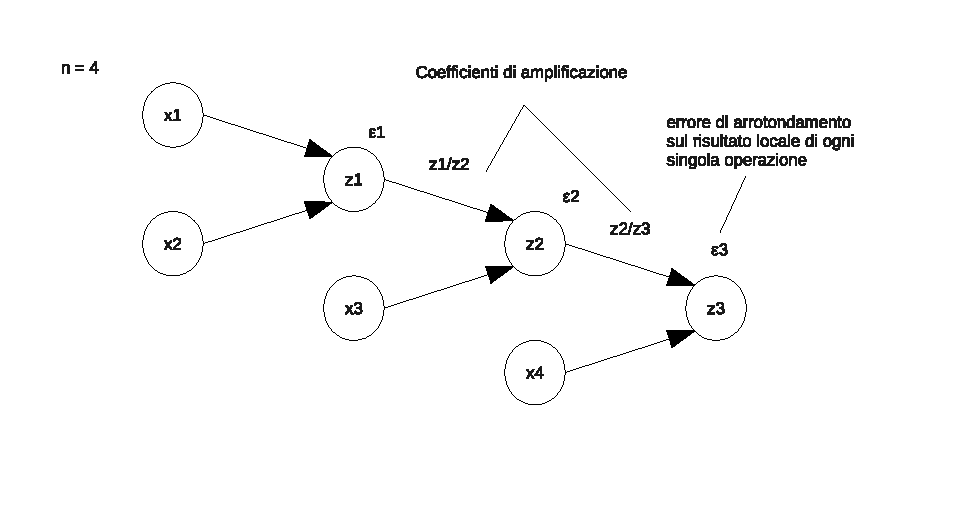
\includegraphics{fig/algoritmo1.eps}
\caption{Algoritmo $1$.}
\end{figure}
\end{flushleft}
Per $n$ addendi l'errore complessivo finale sarà:
\[
\varepsilon^{n-1}= \varepsilon^{(n-1)} + \underbrace{\frac{z^{(n-2)}}{z^{(n-1)}}
\cdot\varepsilon^{n-2}}_{\textrm{errore trascinato dagli addendi}}.
\]
Dove $\varepsilon^{n-2}$ è l'errore complessivo che si è annidato sul 
penultimo nodo del grafo.

\[\varepsilon^{n-1}=\varepsilon^{(n-1)} + \frac{z^{(n-2)}}{z^{(n-1)}} \left(
\varepsilon^{(n-2)} +\frac{z^{(n-3)}}{z^{(n-2)}}\varepsilon^{n-3} \right)\]
\[= \varepsilon^{(n-1)} + \frac{z^{(n-2)}}{z^{(n-1)}}\varepsilon^{(n-2)} +
\frac{z^{(n-3)}}{z^{(n-1)}}\left(\varepsilon^{(n-3)} + \frac{z^{(n-4)}}{z^{(n-3)}}
\right)\]
\[\vdots\]
\[= \varepsilon^{(n-1)} + \frac{z^{(n-2)}}{z^{(n-1)}}\varepsilon^{(n-2)} +
\frac{z^{(n-3)}}{z^{(n-1)}}\varepsilon^{(n-3)} + \cdots + \frac{z^{(1)}}{z^{(n-1)}}
\varepsilon^{(1)} = \frac{1}{z^{(n-1)}}\sum_{i=1}^{n-1}z^{(1)}\varepsilon^{(i)}.
\]

Allora:
\[\varepsilon_{\textrm{alg}} = \frac{1}{f(\underline{x})} \cdot \sum_{i=1}^{n-1}
\left(\sum_{j=1}^{i+1}x_j\right) \cdot \varepsilon^{(i)}.\]

\begin{osse}
In generale \emph{non è possibile} dare \emph{limitazioni} per 
$\varepsilon_{\textrm{alg}}$ che non dipendono dai dati.
\end{osse}

Se $\left\{x_i\right\}$ sono tutti dello stesso segno, vale:
\[\left|\sum_{j=1}^{i+1}x_j\right| \leq \left|f(x)\right|, \quad i = 1, \ldots, 
n-1.\]

Allora:
\[|\varepsilon_{\textrm{alg}}| \leq \frac{1}{|f(\underline{x})|}
\sum_{i=1}^{n-1}\left|f(x)\right| \left|\varepsilon^{(i)}\right| \leq
(n-1)\cdot \verb eps  \qquad \textrm{crescita lineare.}\]

L'algoritmo è numericamente ben condizionato per $n$ piccoli, altrimenti
non lo è. In questo caso cosa possiamo fare?

\subsubsection{Algoritmo 1.2.}
Supponiamo di dare gli addendi in ordine di modulo non decrescente, la 
successione delle medie è ancora in modulo non decrescente:
\[\frac{1}{i}\left|\sum_{j=1}^ix_j\right| \leq \frac{1}{i+1}\left|
\sum_{j=1}^{i+1}
x_j\right| \leq \frac{1}{n}|f(\underline{x})|.\]

Allora:
\[|\varepsilon_{\textrm{alg}}| \leq \frac{1}{|f(\underline{x})|}\cdot 
\sum_{i=1}^{n-1}\left|\sum_{j=1}^{i+1}x_j\right| \cdot |\varepsilon^{(i)}| \leq 
\frac{1}{|f(\underline{x})|}\sum_{i=1}^{n-1}\frac{(i+1)f(\underline{x})}{n}
\cdot \verb eps =
\]
\[= \frac{eps}{n} \sum_{i=1}^{n-1}(i+1) < \frac{n+1}{2} \cdot\verb eps .\]

\[\longrightarrow \
|\varepsilon_{\textrm{alg}}| < \frac{n+1}{2} \cdot\verb eps \qquad 
\textrm{crescita lineare.}\]

\begin{osse}
La stima è migliorata di un coefficiente $\frac{1}{2}$.
\end{osse}

\subsection{Algoritmo 2.}
Addizioni in parallelo.

Sia $n = 2^p$, con $p$ intero positivo.
\begin{flushleft}\samepage
\textbf{Poniamo:}\\
$v_j^{(0)} = x_j, \quad j = 1, \ldots, n;$\\
$v_j^{(i)} = v_{2j -1}^{(i-1)} + v_{2j}^{i-1}, \quad j = 1, \ldots, \frac{n}{2^i};
\quad i = i, \ldots, p;$\\
$f(\underline{x}) = v_1^{(p)}.$
\begin{figure}[!ht]
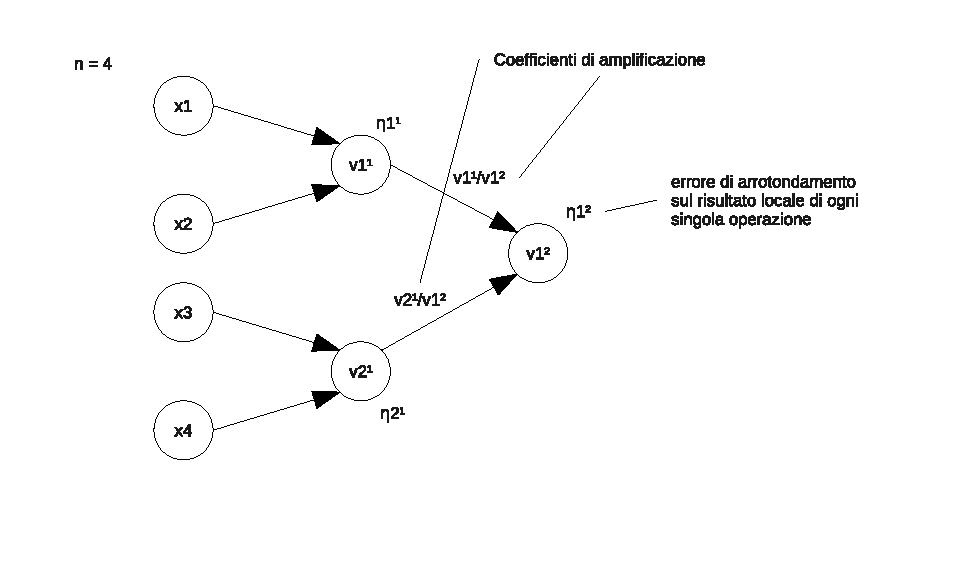
\includegraphics[scale=.75]{fig/algoritmo2.eps}
\caption{Algoritmo $2$.}
\end{figure}
\end{flushleft}
\begin{prop}
L'errore algoritmico è quantificabile come:
\[\varepsilon_{\textrm{alg}} = \frac{1}{f(\underline{x})}\sum_{i=1}^p
\sum_{j=1}^{\frac{n}{2^i}}v_j^{(i)}\eta_j^{(i)}.\]

Poiché, dati gli $x_i$ dello stesso segno, si ha:
\[\sum_{j=1}^{\frac{n}{2^i}}\left|v_j^{(i)}\right| = |f(\underline{x})| 
\quad i = 0,
\ldots, p\]
risulta quindi:
\[|\varepsilon_{\textrm{alg}}| < \max_{i,j}\left|\eta_j^{(i)}\right|\cdot
\sum_{i=1}^p
\sum_{j=1}^{\frac{n}{2^i}}\frac{\left|v_j^{(i)}\right|}{|f(\underline{x})|}
= \max_{i,j}\left|v_j^{(i)}\right|\cdot p < \verb eps \cdot \log_2n.\]

\[|\varepsilon_{\textrm{alg}}| < \verb eps \cdot \log_2n.\]
\end{prop}
\begin{dimo}
Per $n = 2^{k+1}$ addendi l'errore algoritmico complessivo sarà:
\[\varepsilon_{\textrm{alg}} = \eta_1^{k+1} = \eta_1^{(k+1)} + \eta_1^{k} \cdot
\frac{v_1^{(k)}}{v_1^{(k+1)}} + \eta_2^{k}\cdot\frac{v_2^{(k)}}{v_1^{(k+1)}}.\]
\textbf{Ipotesi induttiva:}
\[\eta_1^{k} = \frac{1}{v_1^{(k)}} \cdot \sum_{i=1}^k\sum_{j=1}^{\frac{n}{2^i}^* }
v_j^{(i)}\eta_j^{(i)}, \quad
\eta_2^{k} = \frac{1}{v_2^{(k)}} \cdot \sum_{i=1}^k\sum_{j=1}^{2^{k+1-i}}
v_j^{(i)}\eta_j^{(i)}.\]
Nota $*: \ \frac{n}{2^i} = \frac{2^k}{2^i} = 2^{k-i}$.

\[
\varepsilon_{\textrm{alg}} = \eta_1^{(k+1)} + \frac{1}{\cancel{v_1^{(k)}}} 
\sum_{i=1}^k\sum_{j=1}^{2^{k-i}}v_j^{(i)}\eta_j^{(i)}\cdot
\frac{\cancel{v_1^{(k)}}}{v_1^{(k+1)}} + \frac{1}{\cancel{v_2^{(k)}}}
\cdot \sum_{i=1}^k\sum_{j=1}^{2^{k+1-i}}v_j^{(i)}\eta_j^{(i)} \cdot
\frac{\cancel{v_2^{(k)}}}{v_1^{(k+1)}}
\]

\[
= \frac{1}{v_1^{(k+1)}} \left( 
v_1^{(k+1)}\eta_1^{(k+1)} + \sum_{i=1}^k\sum_{j=1}^{2^{k+1-i}}v_j^{(i)}\eta_j^{(i)}
\right)
\]

\[
=\frac{1}{v_1^{(k+1)}} \cdot \sum_{i=1}^{k+1}\sum_{j=1}^{2^{k+1-i}}v_j^{(i)}\eta_j^{(i)}
.\]

Poiché avevamo posto $f(\underline{x}) = v_1^{(p)}$ con $p = n = k+1$, si ha:
\[
\varepsilon_{\textrm{alg}} = \frac{1}{f(\underline{x})}\sum_{i=1}^p
\sum_{j=1}^{\frac{n}{2^i}}v_j^{(i)}\eta_j^{(i)}.
\]
\end{dimo}
